\documentclass[10pt]{beamer}

\usetheme[progressbar=frametitle]{metropolis}
\usepackage{appendixnumberbeamer}

\usepackage{booktabs}
\usepackage[scale=2]{ccicons}

\usepackage{pgfplots}
\usepgfplotslibrary{dateplot}

\usepackage{xspace}
\newcommand{\themename}{\textbf{\textsc{metropolis}}\xspace}

\usepackage[style=authoryear,backend=biber]{biblatex}
\addbibresource{main.bib}

% Clear the urldate macro entirely
\renewbibmacro*{url+urldate}{}


% Remove all entry prefixes/icons
\DeclareFieldFormat{labelnumberwidth}{}
\renewbibmacro*{begentry}{}
\setbeamertemplate{bibliography item}{}

% Make bibliography text smaller
\renewcommand*{\bibfont}{\tiny}

% Remove unwanted fields
\AtEveryBibitem{%
  %\clearfield{doi}%
  \clearfield{eprint}%
  \clearfield{url}%
  \clearfield{urldate}%
  \clearfield{isbn}%
  \clearfield{issn}%
}

% Configure footnote citations
\DeclareCiteCommand{\footcite}[\mkbibfootnote]
  {\usebibmacro{prenote}}
  {\usebibmacro{citeindex}%
   \printtext[bibhyperref]{\usebibmacro{cite}}}
  {\multicitedelim}
  {\usebibmacro{postnote}}

% Make footnotes smaller
\setbeamerfont{footnote}{size=\tiny}

% Mark smaller captions
\setbeamerfont{caption}{size=\tiny}

\title{Catching Stray Balls}
\subtitle{Football, fandom, and the impact on digital discourse}
% \date{\today}
\date{25 June 2025}
\author{Mark J. Hill}
\institute{Department of Digital Humanities, KCL}
\titlegraphic{
    \vspace*{\fill}
    \hspace*{\fill}
    
\includegraphics[height=1.5cm]{King's_College_London_Digital_Humanities.png}
    \hspace{0cm}  % Optional: add some margin from the edge
    \vspace{-8.5cm}  % Optional: add some margin from the bottom
}

\begin{document}

\maketitle

%%\begin{frame}{Table of contents}
%%  \setbeamertemplate{section in toc}[sections numbered]
%%  \tableofcontents%[hideallsubsections]
%%\end{frame}

%%\section[Intro]{Introduction}

\begin{frame}{The question and why it matters}

\begin{columns}
\begin{column}{0.55\textwidth}
\begin{itemize}
\item \textbf{Research Question:}
Do real-world events trigger toxic behaviour that spreads across unrelated online communities?
\item \textbf{Approach:} Football as a 'natural experiment' with clear, time-stamped emotional triggers

\item \textbf{Process:}
{\small
    \begin{enumerate}
    \item Identify a method for measuring toxicity
    \item Identify a cause of toxicity
    \item Measure the movement of toxicity
    \item Examine toxic content
    \end{enumerate}
}

\end{itemize}
\end{column}

\begin{column}{0.55\textwidth}
\textbf{Why This Matters}
\item Users encountering toxic online discourse experience negative psychological consequences. \footcite{braghieri_social_2022, allcott_welfare_2020}
\item Social media affordances amplify this emotional content. \footcite{milli_engagement_2025, kramer_experimental_2014, tsugawa_negative_2015} 
\item Those exposed to emotionally charged social media (positive and negative) are more likely to express similar sentiments. \footcite{ferrara_measuring_2015, Brady_2017}

\end{column}
\end{columns}
\end{frame}

%%\section{The Dataset}

\begin{frame}{The datasets}

\begin{columns}
\begin{column}{0.6\textwidth}
\begin{itemize}
\item \textbf{Scale:} 62+ million Reddit posts from 41 football club subreddits (2008-2024)
\item \textbf{Matched Events:} 20,764 actual match results with kick-off time for aligning with posts
\item \textbf{Cross-Community:} Half a million pairs of posts made by same users in football and non-football subreddits within 10-minute window
\end{itemize}
\end{column}
\begin{column}{0.4\textwidth}
\centering
  \begin{table}
    \resizebox{\columnwidth}{!}{
      \begin{tabular}{lrrrr}
        \hline
        \textbf{Match Result} & \textbf{Posts} & \textbf{\%} \\
        \hline
        Wins & 6,477,964 & 49.6\\
        Draws & 2,690,511 & 20.6 \\
        Losses & 3,902,686 & 29.9 \\
        Total & 13,071,161 & 100 \\
        \hline
      \end{tabular}
    }
    \caption{Match-aligned posts overview.}
    \label{tab:match_posts}
  \end{table}
\end{column}
\end{columns}
    
\end{frame}

%% \section{Elements}

\begin{frame}{Finding 1: Negativity = Toxicity}

\begin{columns}
\begin{column}{0.67\textwidth}

How do we measure toxicity?

\begin{itemize}
\item Used RoBERTa-based sentiment and toxicity detection, and the "List of dirty, naughty, obscene, and otherwise bad words" lexicon.\footcite{camacho-collados_tweetnlp_2022, nicholas22aira, LDNOOBW2025}
\item Strong correlation between negative sentiment and problematic content

\item Effect sizes: Hate speech (δ = -0.5), Toxicity (δ = -0.47)
\end{itemize}

\textbf{Implication:} Sentiment can serve as an early warning signal for toxic content
\end{column}

\begin{column}{0.33\textwidth}

\begin{figure}[t]
    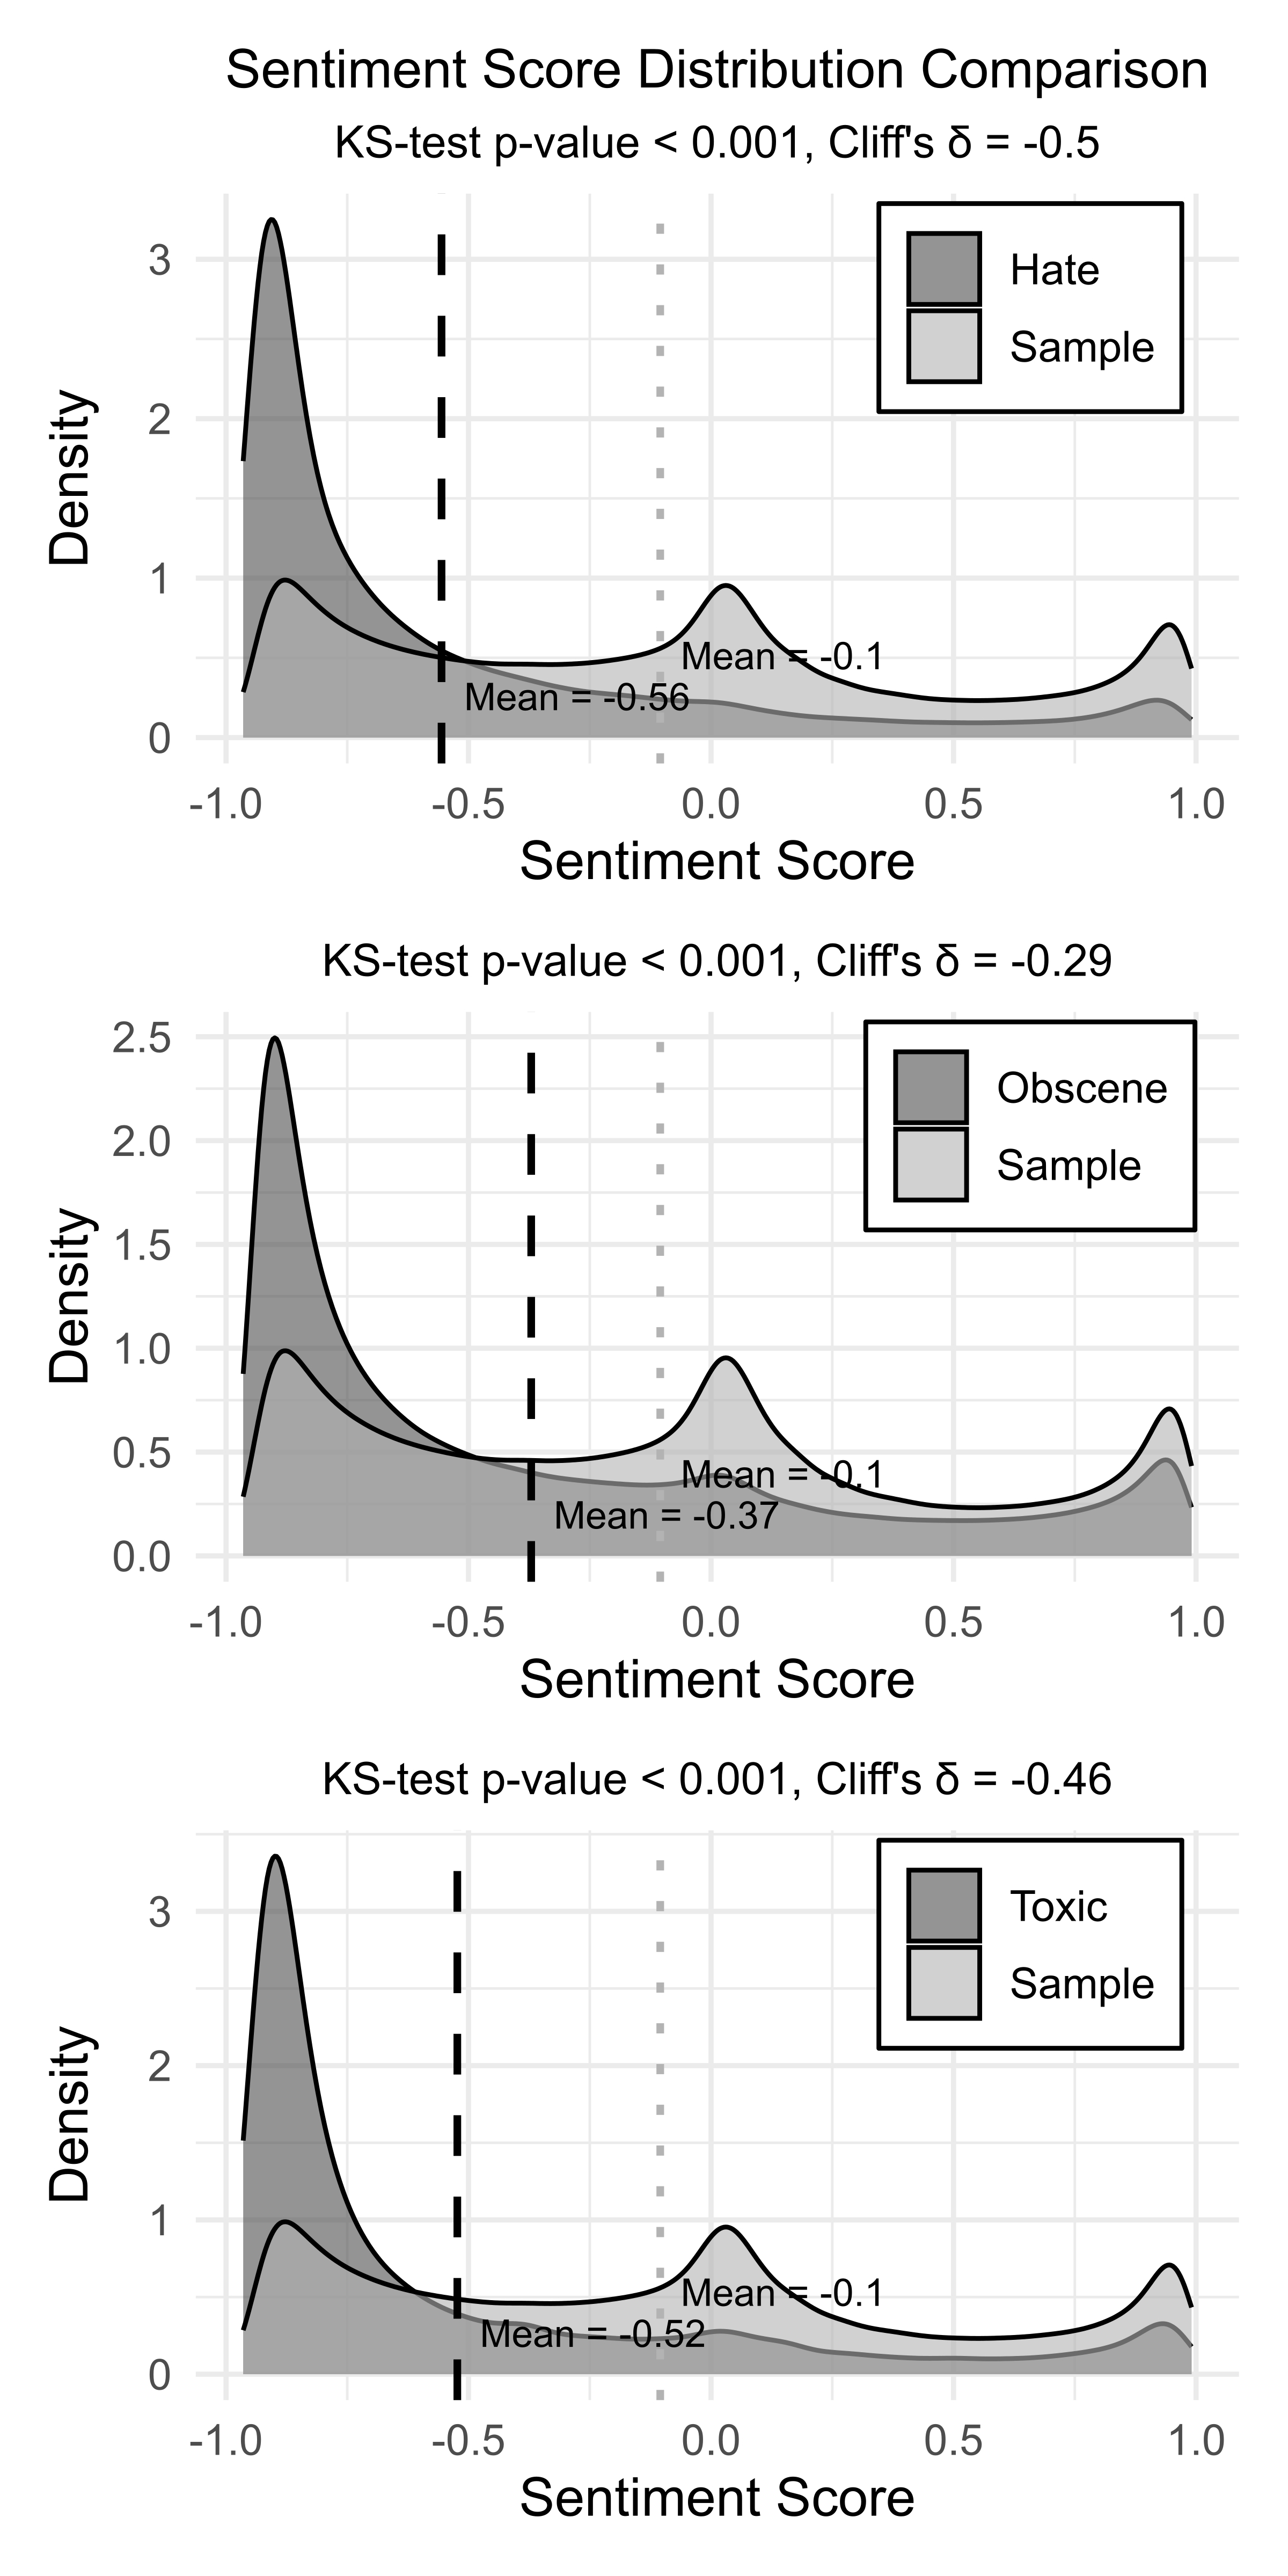
\includegraphics[width=\columnwidth]{combined_density_plots_with_legend_600dpi.jpg}
    \caption{Comparative sentiment score distributions.}
    \label{fig:density_plots}
\end{figure}

\end{column}
\end{columns}
\end{frame}


\begin{frame}{Finding 2: Football results drive online sentiment}

\begin{columns}
\begin{column}{0.7\textwidth}
\begin{table}
\centering
\resizebox{\columnwidth}{!}{%
\begin{tabular}{lccc}
\hline
\textbf{Result} & \textbf{Posts per match} & \textbf{Post ratio} & \textbf{Average Sentiment} \\
\hline
\multicolumn{4}{l}{\textit{Within 120 Minutes of Kick-off}} \\
Loss & 739.32 & 0.89*** & -0.25*** \\
Draw & 764.37 & 0.92*** & -0.11*** \\
Win  & 934.13 & 1.12*** &  0.07*** \\
\hline
\multicolumn{4}{l}{\textit{Within 8 Hours of Kick-off}} \\
Loss & 577.14 & 0.80*** & -0.17*** \\
Draw & 604.96 & 0.84*** & -0.09*** \\
Win  & 904.49 & 1.26*** &  0.06*** \\
\hline
\end{tabular}%
}
\caption{Posting volume and sentiment in FC subreddits following different match results reveal an asymmetric emotional response.}
\label{tab:match_results_combined}
\end{table}

\textbf{Asymmetric Effect: }
Losses decrease sentiment and number of posts; wins increase posts, but have a comparatively small impact on sentiment.

\textbf{Causal Evidence:} Clear temporal relationship between events and sentiment shifts

\end{column}
\begin{column}{0.3\textwidth}
\centering

\begin{figure}[t]
    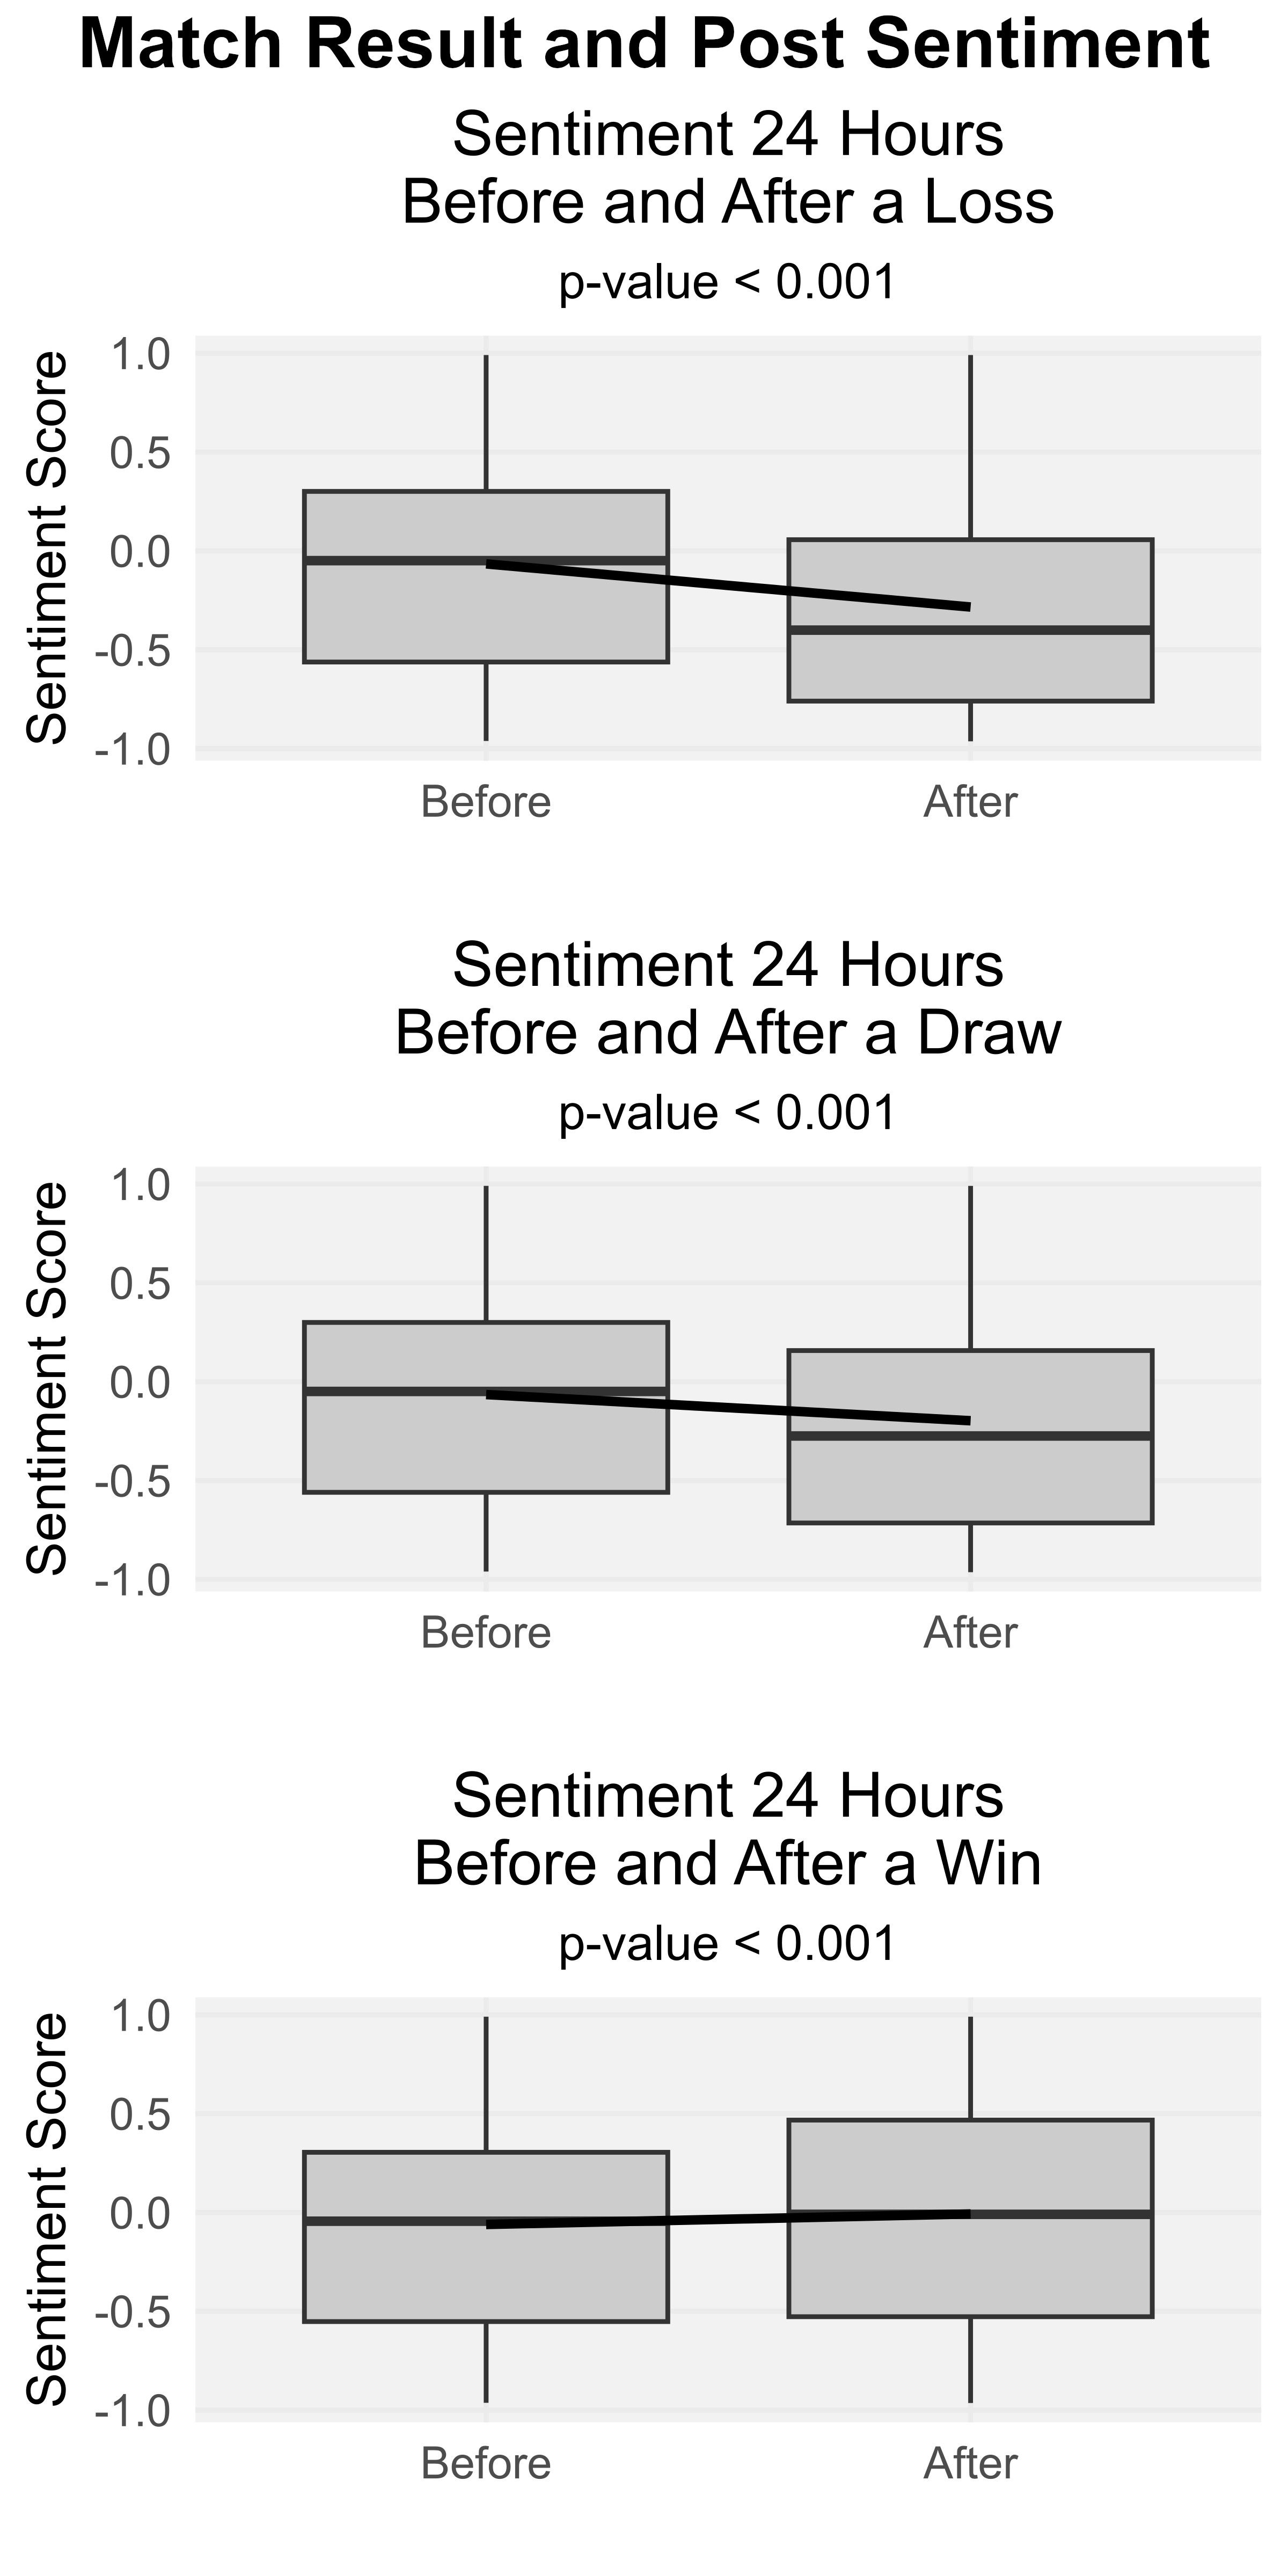
\includegraphics[width=\columnwidth]{sentiment_before_after_matches_600dpi.jpg}
    \caption{Change in poster sentiment over 48-hour period around kick-off (FC Corpus).}
    \label{fig:sentiment_change_24}
\end{figure}

\end{column}
\end{columns}

\end{frame}

\subsection{Micro}
\begin{frame}{Micro}
\begin{columns}
\begin{column}{0.5\textwidth}
\begin{figure}
    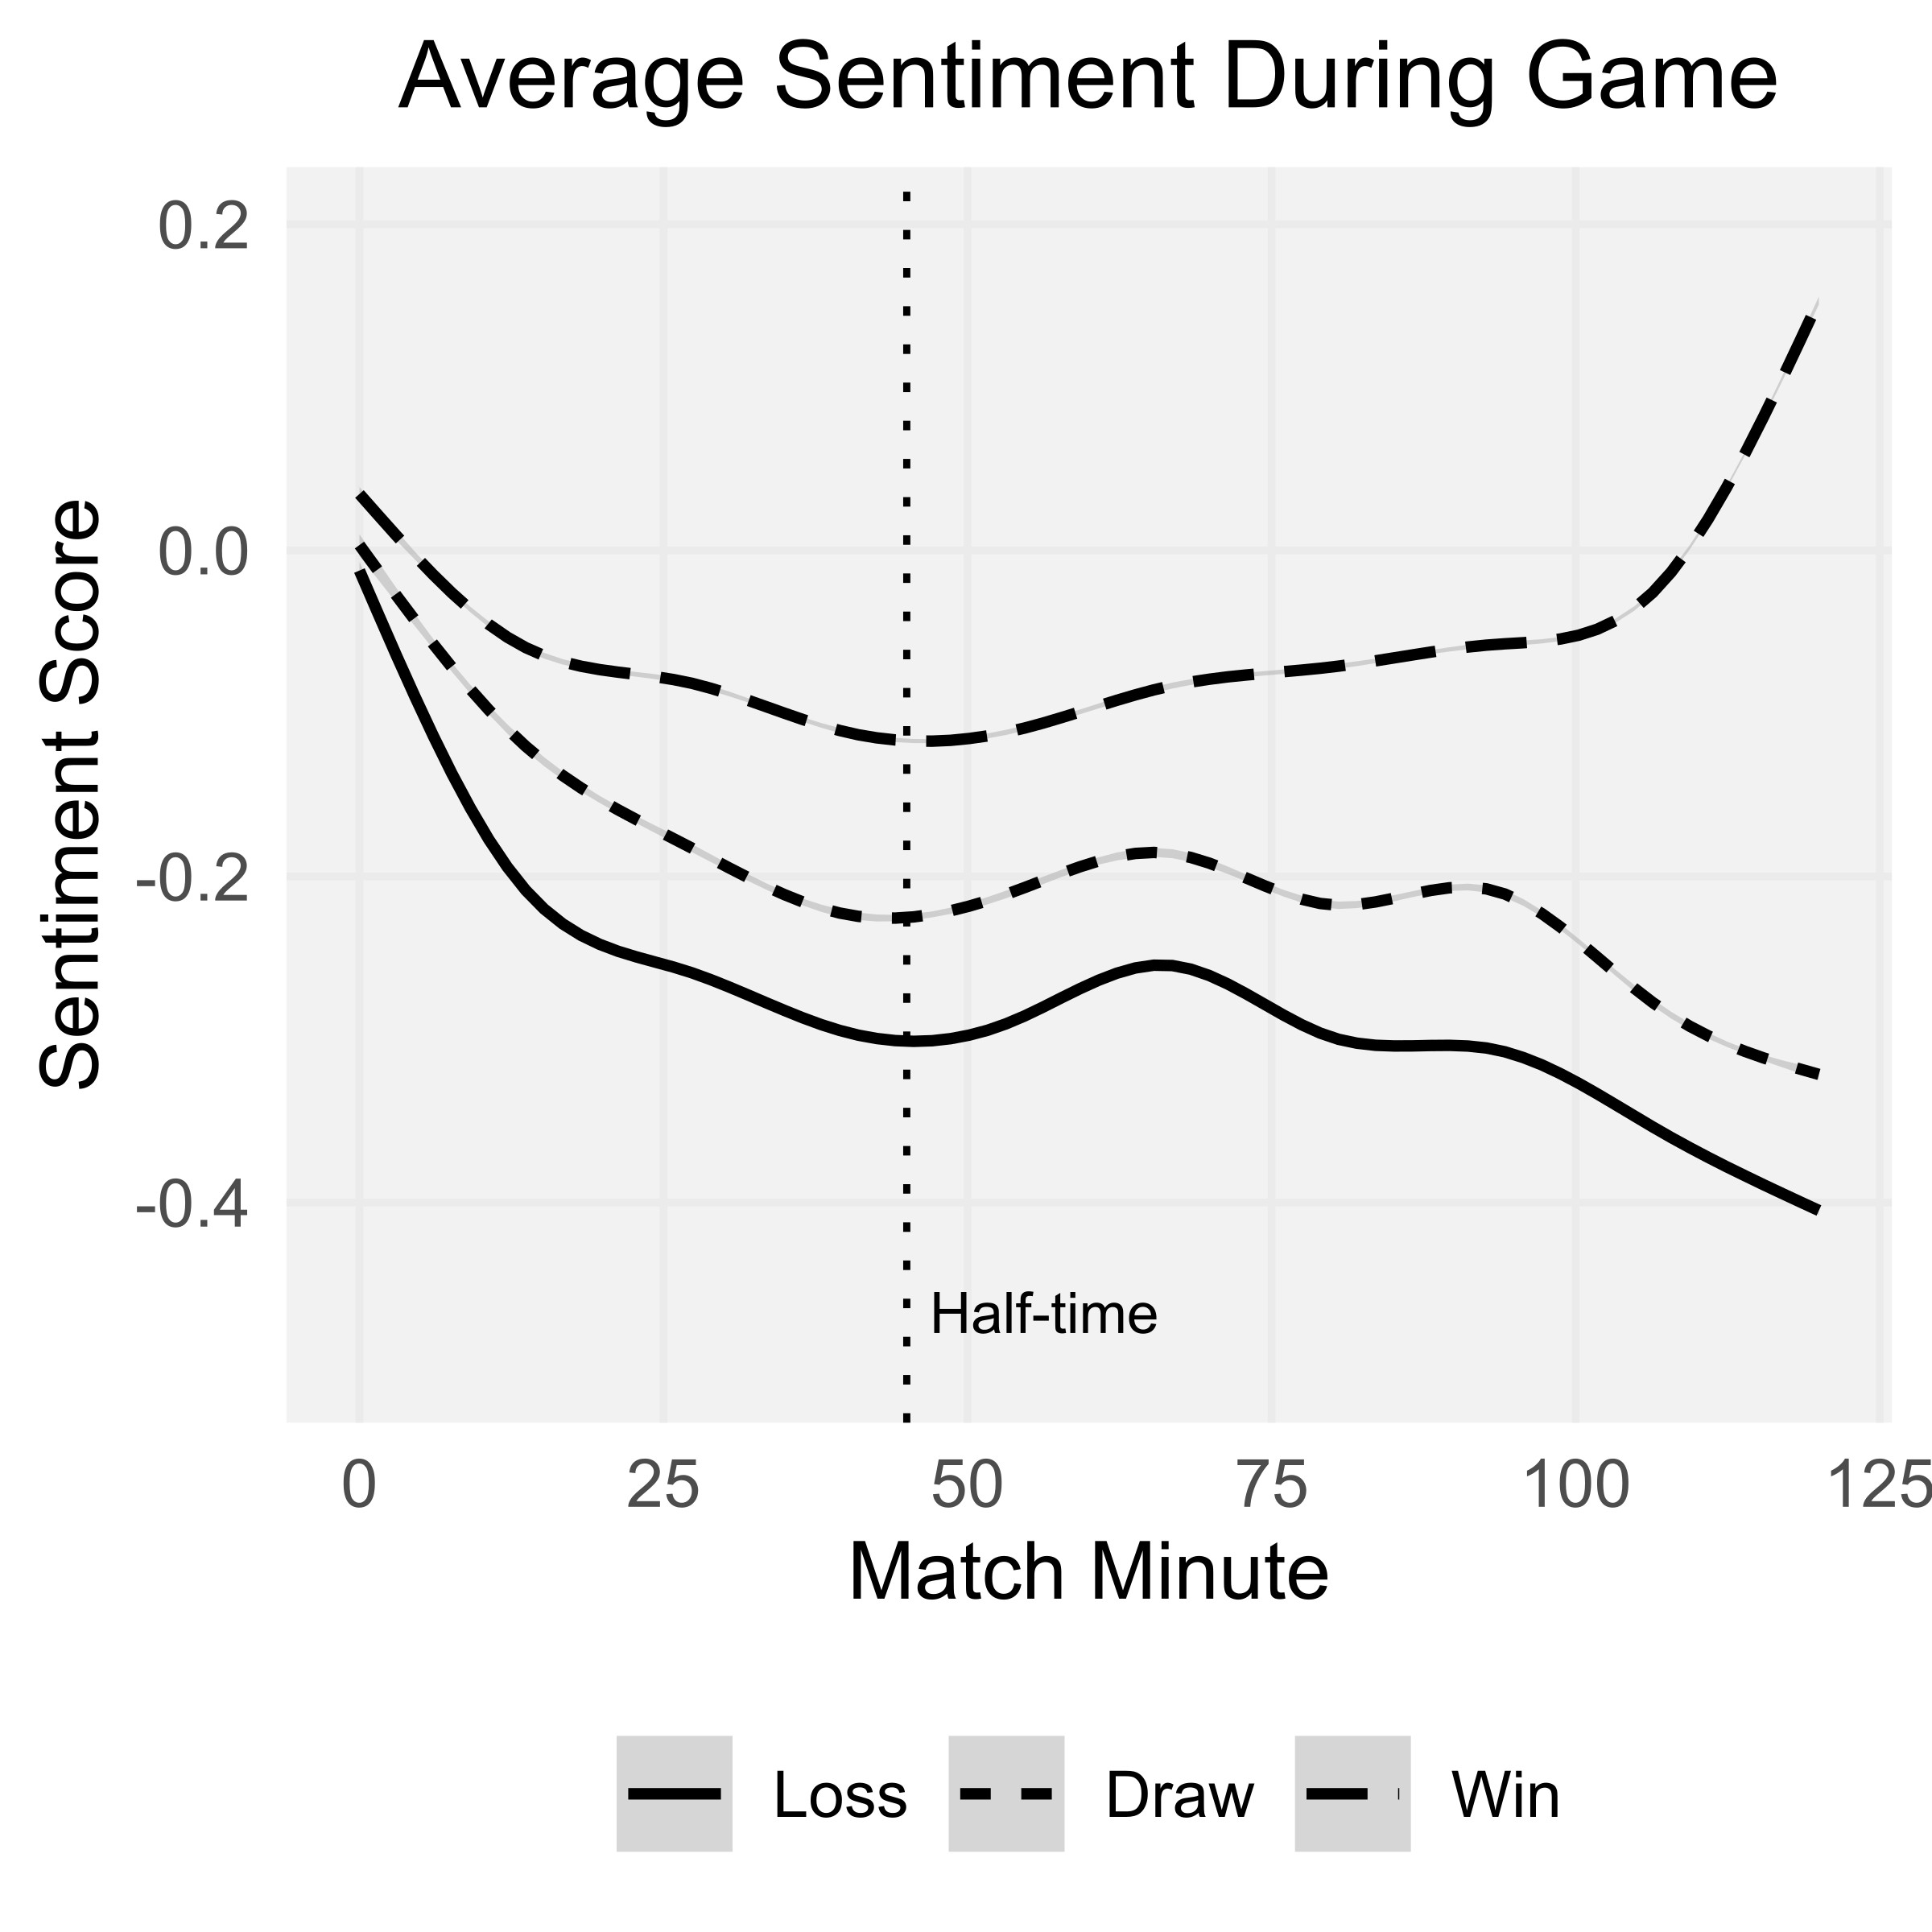
\includegraphics[width=\columnwidth]{sentiment_during_match_small_600dpi.jpg}
    \caption{Aggregated sentiment change per-minute by match result (FC Corpus).}
    \label{fig:sentimentchange}
\end{figure}
\end{column}
\begin{column}{0.5\textwidth}
\begin{figure}
    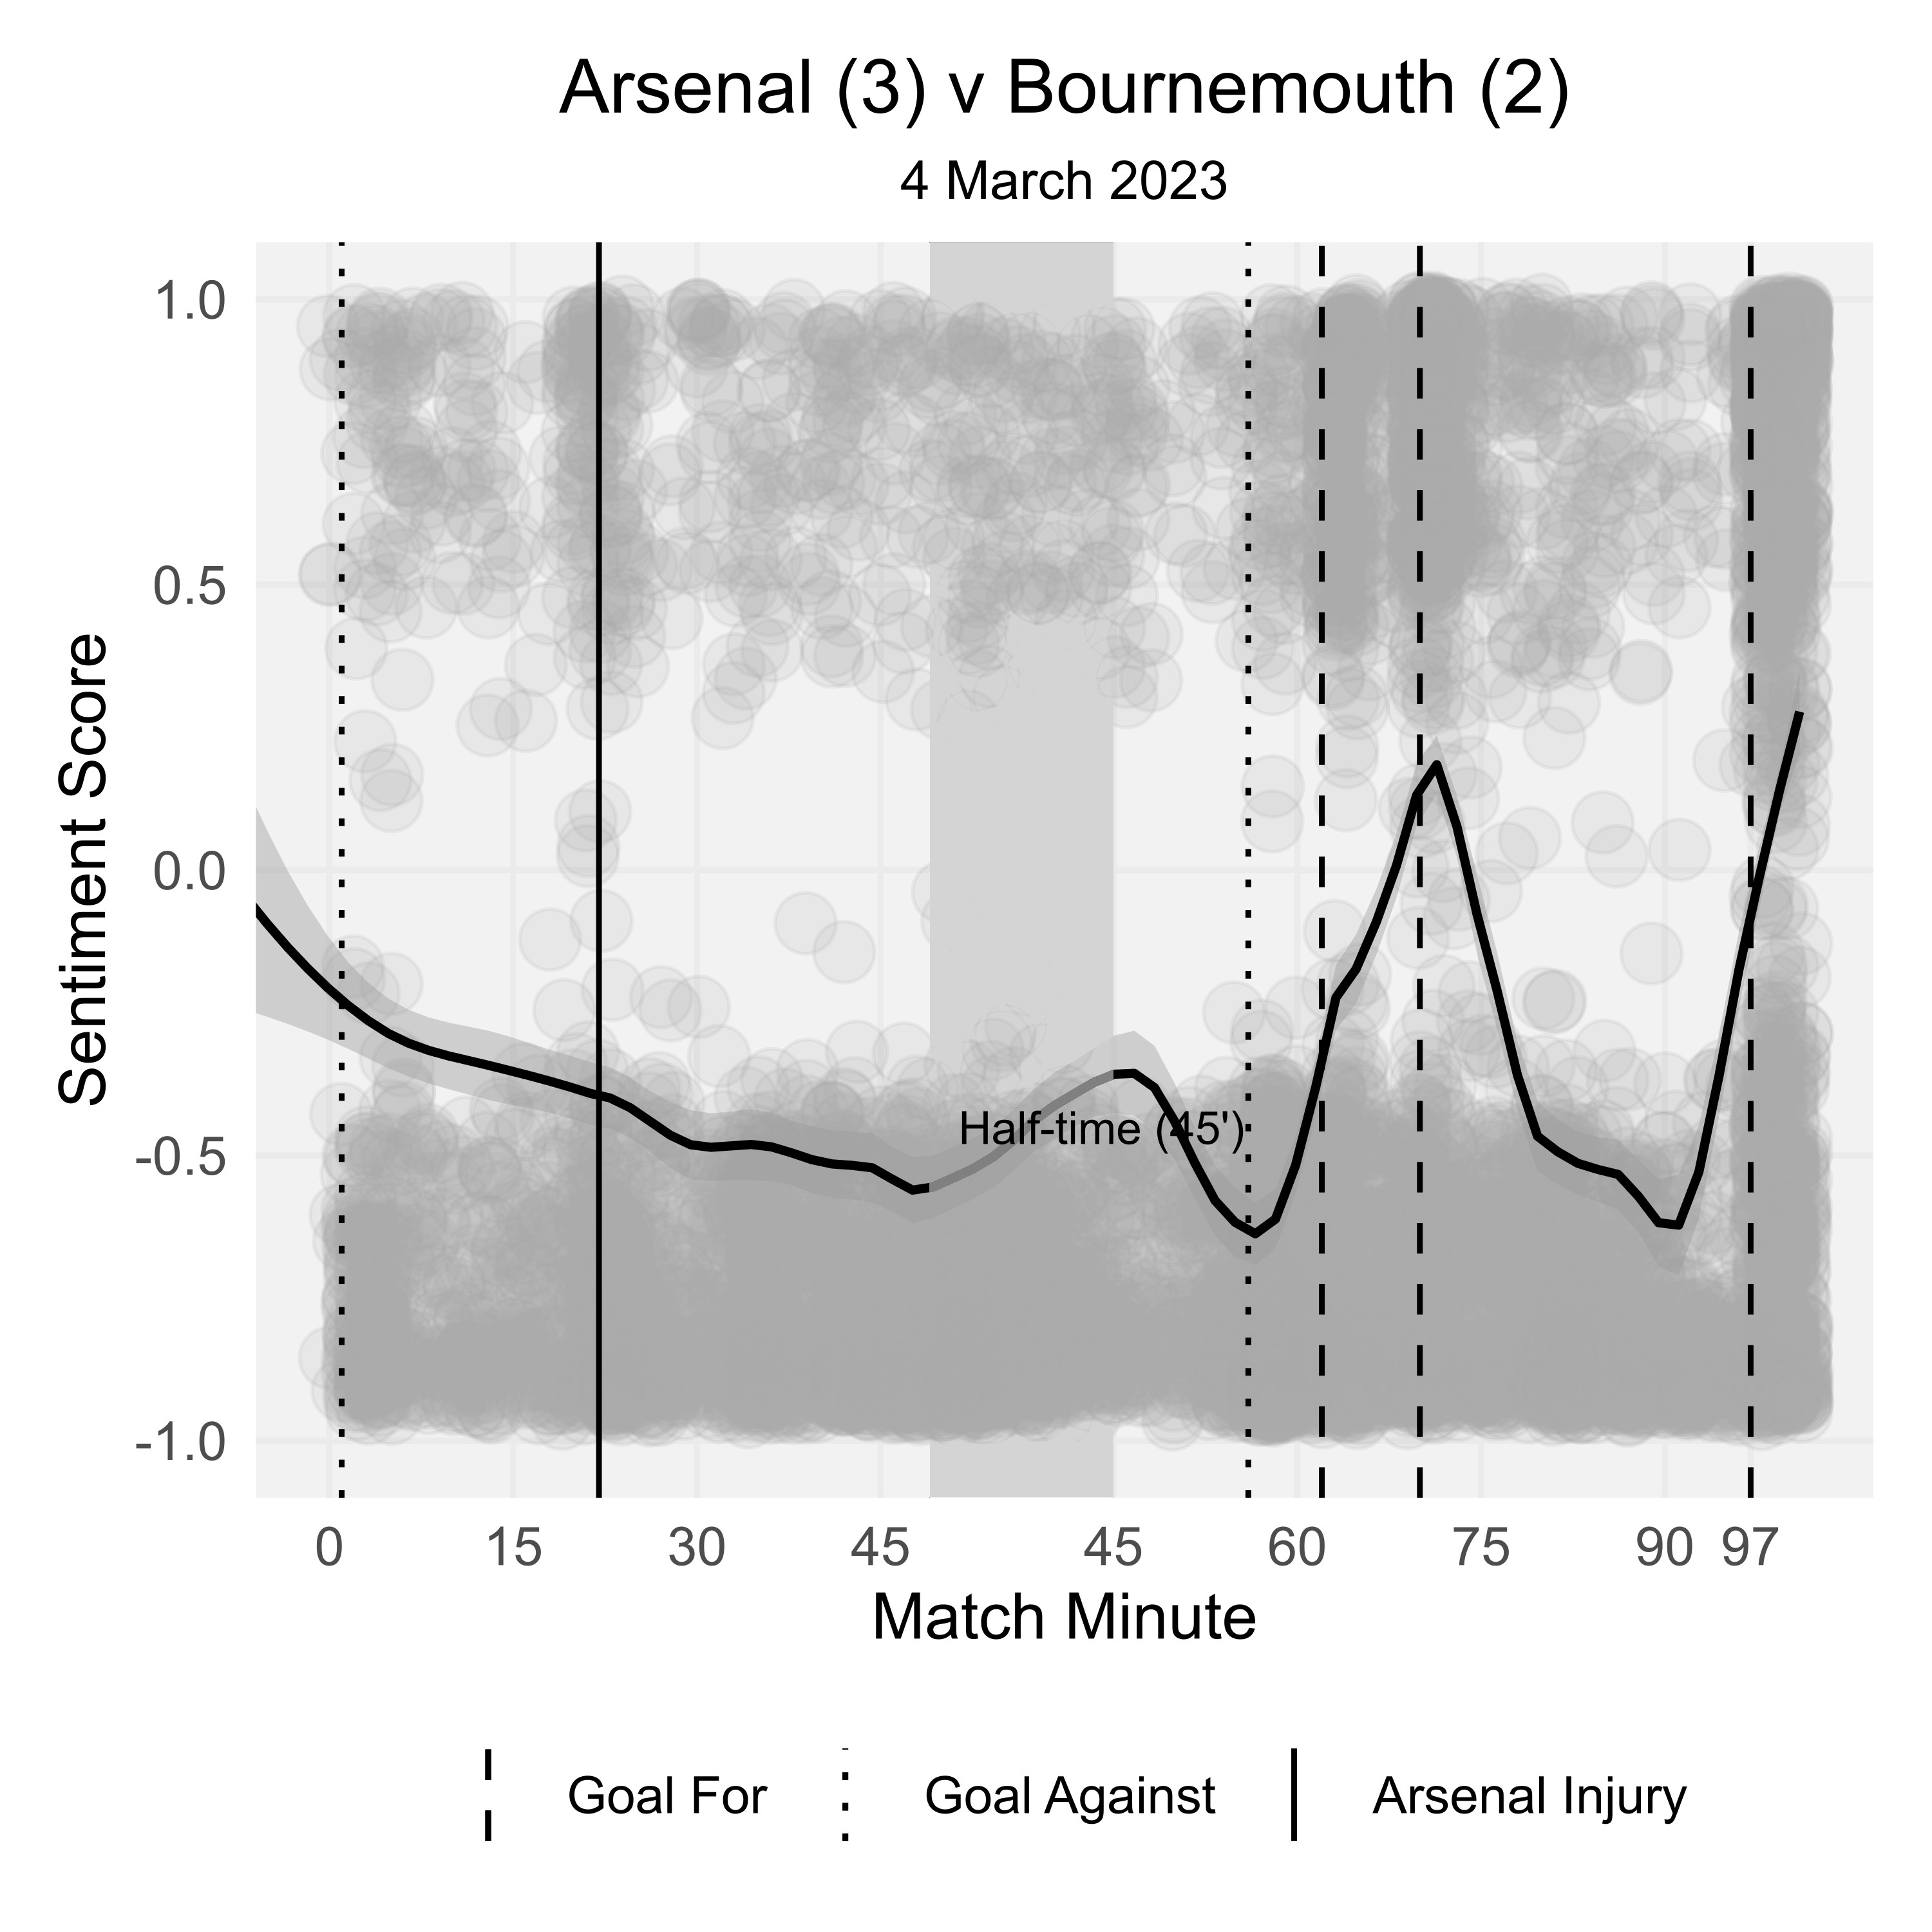
\includegraphics[width=\columnwidth]{sentiment_specific_game_small_600dpi.jpg}
    \caption{Post sentiment during Arsenal-Bournemouth match. Neutral posts removed to aid visualisation.}
    \label{fig:arsenal_bournmouth}
\end{figure}
\end{column}
\end{columns}
\end{frame}

\subsection{Macro}
\begin{frame}{Macro}
\begin{figure}
    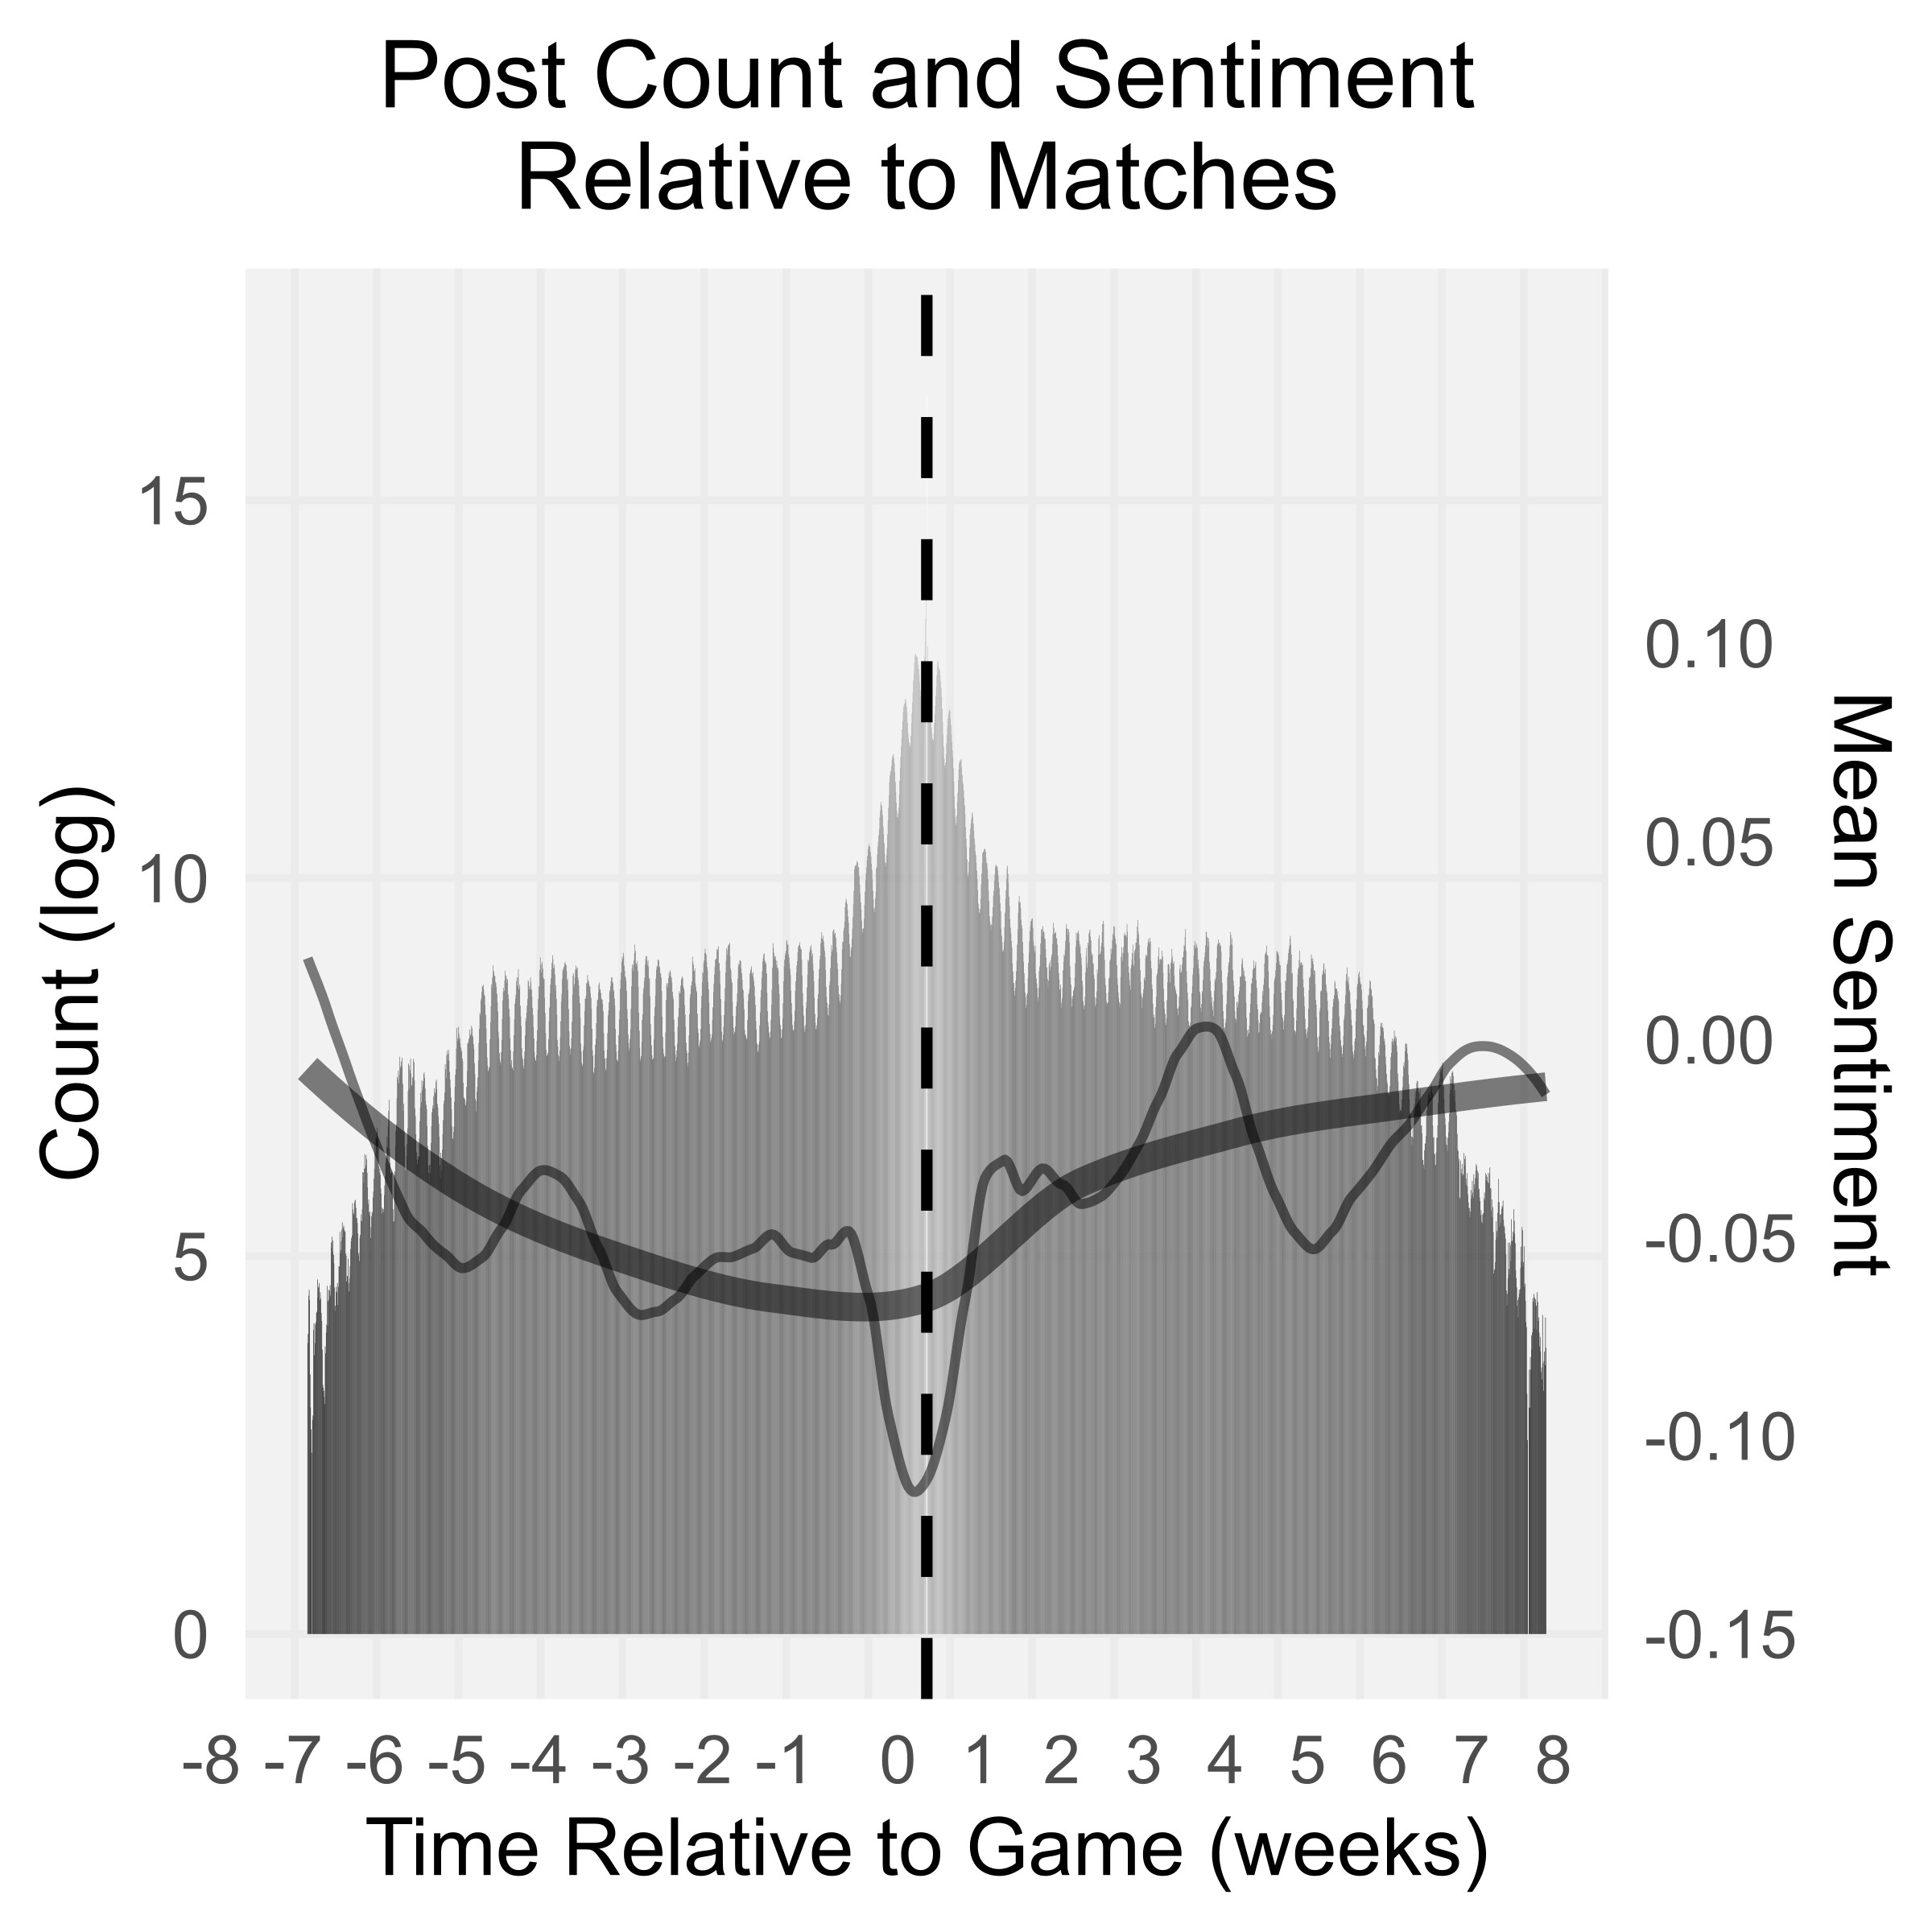
\includegraphics[width=\textwidth,height=0.8\textheight,keepaspectratio]{sent_v_weeks_to_match_small_600dpi.jpg}
    \caption{Post count (log) and sentiment relative to game (FC Corpus).}
    \label{fig:sentimentchange}
\end{figure}
\end{frame}




\begin{frame}{Finding 3: Emotional spillover across communities}

\begin{columns}
\begin{column}{0.55\textwidth}
Emotional states in football subreddits predict sentiment in unrelated subreddits.

\begin{itemize}
\item \textbf{Baseline correlation:} $\tau$ = 0.059
\item \textbf{During matches:} $\tau$ = 0.118 (doubles!)
\item \textbf{Evidence:} Matching sentiment occurs more than chance
\item \textbf{Impact:} Hundreds of thousands of cross-community interactions affected
\end{itemize}

When neutral posts are removed correlations increase further ($\tau$ 0.146).
\end{column}

\begin{column}{0.45\textwidth}
\centering

\begin{table}[ht]
\centering
\resizebox{\columnwidth}{!}{%
\begin{tabular}{lrr}
\hline
\textbf{Time Comparison} & \textbf{Kendall's} $\boldsymbol{\tau}$ & \textbf{n} \\
\hline
All Paired Posts & 0.085*** & 575,863 \\
During Match & 0.118*** & 234,024 \\
Outside Match & 0.059*** & 341,839 \\
\hline
\end{tabular}%
}
\caption{Kendall's $\tau$ correlation for the sentiment of paired posts by the same user.}
\label{tab:sentiment_correlations_combined}
\end{table}

\begin{table}
  \centering
  \resizebox{\columnwidth}{!}{
    \begin{tabular}{lrrr}
     \hline
    \makecell{\textbf{ }} & \makecell{\textbf{Negative}} & \makecell{\textbf{Neutral}} & \makecell{\textbf{Positive}} \\
    \hline
    \makecell{\textbf{Negative}} & 40.00 & -18.76 & -26.73 \\
    \makecell{\textbf{Neutral}} & -18.92 & 22.74 & -7.59 \\
    \makecell{\textbf{Positive}} & -27.49 & -5.12 & 44.66 \\
    \hline
    \end{tabular}
  }
  \caption{Pearson $\chi$² standardised residuals for paired sentiment categories.}
  \label{tab:chi-2-test}
\end{table}


\end{column}
\end{columns}
\end{frame}

\begin{frame}{Finding 4: Linguistic spillover}
\begin{columns}
\begin{column}{0.45\textwidth}
\textbf{Method:} Analysed language features in paired negative posts
{\footnotesize
\begin{itemize}
\item Profanity (LDNOOBW lexicon)
\item Violent words (kill, attack, destroy, etc.)
\item Intensifiers (very, extremely, f**king, etc.)
\item Exclamation marks (!)
\item ALL-CAPS text
\end{itemize}
}

\vspace{0.5em}
\textbf{Key Finding:} While linguistic features between paired posts already (weakly) correlated, all patterns strengthened during matches.

\end{column}

\begin{column}{0.55\textwidth}
\begin{table}
\centering
\resizebox{\columnwidth}{!}{%
\begin{tabular}{lccc}
\hline
\textbf{Feature} & \textbf{Outside Match} & \textbf{During Match} & \textbf{Difference ($\Delta \tau$)} \\
\hline
Profanity & 0.061*** & 0.109*** & 0.048*** \\
Violent & 0.022*** & 0.049*** & 0.027*** \\
Intensifiers & 0.059*** & 0.074*** & 0.015*** \\
Exclamations & 0.124*** & 0.154*** & 0.035*** \\
All-caps & 0.052*** & 0.133*** & 0.081*** \\
\hline
\end{tabular}%
}
\caption{Linguistic spillover between FC and non-FC subreddits.}
\label{tab:lang_tau_difference}
\end{table}

\textbf{Implication:} Heightened emotional states from football events intensify toxic communication patterns across unrelated digital spaces.

\end{column}
\end{columns}

\end{frame}

\begin{frame}{Examples}

{\footnotesize
\begin{table}[htbp] % Added [htbp] for float placement suggestion
  \centering
  \begin{tabular}{p{.45\linewidth} p{.5\linewidth}}
    \hline
    \textbf{FC Subreddit} & \textbf{Non-FC Subreddit} \\
    \hline
    "F**k our attack is completely useless" & 
    "haha you're such a f****t" (r/filmclips), "this is pure garbage" (r/photoeditbattles) \\
    "I've already told you to get f**cked you absolute c**t. Go finger your ma you pathetic f**k" & 
    "Looks like a total c*m stain that's going to produce more useless human s**t like yourself" (r/VintagePhotos), "She's ignoring you because you're a B***H" (r/maledatingadvice) \\
    "F**k this is bulls**t" & "Eat s**t and die" (r/cambridge) \\
    "F**k off, already. Seriously, f**k off" & "Only a r****d would like this" (r/humor) \\
    "f**k. off. useless. defender." & "I hope someone violently r***s her when she gets home (r/embarrassing) \\
    "The match fell apart when our 2-goal lead vanished because that useless goalkeeper's f**cking error." & "seriously, look at how she's dressed, total s**t" (r/elegantcelebrities) \\
    "this is f**king our team, THIS IS OUR TEAM, WHAT A TOTAL GROUP OF F**KING MUPPETS" & "How can she be happy with herself when she's a disgusting piece of human trash?" (r/SocialMediaScreenshots) \\
    \hline
  \end{tabular}
  \caption{Paired comments from the same author made within 10 minutes. Quotes and subreddits modified to avoid identification.}
  \label{tab:bad_pairs}
\end{table} % Closing the table environment
}
\end{frame}

\begin{frame}{The Mechanism}
\begin{center}
\large
Emotional trigger (e.g., football match)
\\ $\downarrow$ \\
\fbox{\parbox{0.4\textwidth}{\centering 
{\footnotesize \textit{[Identification process]}}\\
Emotional response in relevant community 
\\ $\downarrow$ \\
User moves to unrelated community}}
\\ $\downarrow$ \\
Emotional state transfers 
\\ $\downarrow$ \\
Toxic behavior spreads
\end{center}

Digital communities are not isolated --- they're interconnected emotional ecosystems
\end{frame}

\begin{frame}{Implications \& Applications}
\begin{columns}
\begin{column}{0.5\textwidth}

\textbf{For Research:}
\begin{itemize}
\item Methodology applicable beyond football (elections, breaking news, etc.)
\item Measure cascade effects ('true' emotional contagion)
\end{itemize}

\textbf{For Platform Design:}
\begin{itemize}
\item Predictive moderation during high-risk events
\item Early warning systems through platform monitoring
\end{itemize}

\end{column}
\begin{column}{0.5\textwidth}

\textbf{For Society:}
\begin{itemize}
\item Understanding offline to online harm pathways
\item Hidden mechanisms of toxicity propagation
\end{itemize}

\begin{block}{Broader Impact}
Computational evidence of real-world event-driven emotional spillover across unrelated digital communities
\end{block}
\end{column}
\end{columns}
\end{frame}


\appendix

\begin{frame}
\centering
\Huge Thank you!

\vspace{1em}
\Large Questions?

\vspace{2em}
\normalsize
\texttt{mark.j.hill@kcl.ac.uk}\\
\textbf{Pre-print:} \textit{doi.org/10.48550/arXiv.2506.01642}\\
\textbf{Repo:} \textit{github.com/markjhill/2025-catching-strays}
\end{frame}

\begin{frame}[allowframebreaks]{References}
  \printbibliography
\end{frame}

\begin{frame}[fragile]{Backup slides}
  Sometimes, it is useful to add slides at the end of your presentation to
  refer to during audience questions.

  The best way to do this is to include the \verb|appendixnumberbeamer|
  package in your preamble and call \verb|\appendix| before your backup slides.

  \themename will automatically turn off slide numbering and progress bars for
  slides in the appendix.
\end{frame}

\begin{frame}{Blocks}
  Three different block environments are pre-defined and may be styled with an
  optional background color.

  \begin{columns}[T,onlytextwidth]
    \column{0.5\textwidth}
      \begin{block}{Default}
        Block content.
      \end{block}

      \begin{alertblock}{Alert}
        Block content.
      \end{alertblock}

      \begin{exampleblock}{Example}
        Block content.
      \end{exampleblock}

    \column{0.5\textwidth}

      \metroset{block=fill}

      \begin{block}{Default}
        Block content.
      \end{block}

      \begin{alertblock}{Alert}
        Block content.
      \end{alertblock}

      \begin{exampleblock}{Example}
        Block content.
      \end{exampleblock}

  \end{columns}
\end{frame}



\end{document}
